\chapter{Higher Order Applications: Multiple Object Tracking}

As the final aim of my thesis, I am going to inspect the performance of the chosen object detectors on a higher-order problem (meaning that detection is only the first conceptual layer of the solution), namely multiple object tracking (MOT). First I am going to review the problem itself, and the common metrics used to measure its performance. 

After this, I will elaborate on the object tracker implementation I chose as the basis, showing how it incorporates the aforementioned detectors, and the way the performance of the latter is expected to influence tracking performance.

Finally, I will describe my experimental setup aiming to measure tracker performance based on the detector type supplied to it. Several parts of the evaluation environment were implemented by me, so I will detail my design chices whenever such a part comes into focus.

\section{The problem and possible approaches}

Multiple object tracking (MOT) consists of determining the \textit{trajectory} of given kinds of objects in a video stream. In the current context, the trajectory of a single, unique object is a series of bounding boxes with an identifier, one box for every frame in which the object is visible. The rectangular bounding boxes are expected to fit the object shilouette as tightly as possible.

Along the years, several approaches have been developed for the problem, but with the advent of highly accurate object detectors (most notably the breakthrough of convolutional neural networks from the mid-2010s and onward), the detection-based paradigm has become one of the most popular.

The approach consists of detecting objects on each new frame, then assigning them to previously found trajectories, if the object has been seen before, or registering a new trajectory otherwise. This is generally called the \textit{association step}. In some scenarios, when the objects of interest are densely packed, this can pose a considerable difficulty.

Among some popular solutions to this association problem are the \textit{proximity-based} (the Simple Online and Realtime Tracking (SORT) architecture~\cite{Bewley_2016} is one example) and the \textit{feature-based} (the DeepSORT architecture \cite{DeepSORT} incorporates such methods using \textit{deep appearance descriptors}) assignments. The former considers each already existent trajectory, takes their previous location, or the predicted location for this time step, and does the assignment based on some spatial distance between these and current detections. The latter does overarching associations based on visual appearance features, not necessarily restricted to the appearance observed in the last few frames.

The weakness of the proximity-based approach is when the density of objects is high, their movement highly dynamic and their trajectories intertwined. In this case, feature-based methods might excel. The weakness of the feature-based methods might show when they confuse similar, but distinct objects, or when they cannot account for some drastic, fast changes in appearance (like changes in lighting, orientation, deforming, or partial occlusion). In these situations, assignment to last known locations can help. Thus, these two approaches are not, and should not be exclusive.

The introduction above focuses on paradigms and aspects mostly relevant for my thesis, and narrows down the field somewhat. For a comprehensive, recent overview of the problem, see the literature review at~\cite{Luo_2021}. It goes beyond just the detection-based approach, and also formalises the general problem.

Finally, it is worth mentioning that the most common multi-object tracking targets are pedestrians, faces and vehicles, and thus most popular MOT datasets consist of these. In this thesis, I am going to tackle tracking vehicles in road traffic footages.

\section{Metrics}

When thinking about assessing the performance of multiple object tracking applications, there is no one singular metric that comes to mind, but there are several ways in which a tracker can be wrong (at least in as many ways as an object detector). Starting from these errors, categorizing and counting them, and then inspecting their relation to the total of ground truth detections can give the right picture.

After inspecting some research literature in MOT, I saw that the most popular metrics coming up again and again were the CLEAR MOT metrics, or at least some of them. They were introduced in~\cite{Bernardin2008}, back in 2008, when generally-agreed upon metrics were not estabilished in the field. It proposes the MOTA and MOTP metrics as a way to quantify identity tracking and localization performance.

The CLEAR MOT paper provides not only the metrics themselves, but also explains the specifics of the evaluation process. After a literature and research review, it starts by defining the characteristics of a desirable tracker: `It should at all points in time find the correct number of objects present; and estimate the position of each object as precisely as possible (note that properties such as the contour, orientation, or speed of objects are not explicitly considered here). It should also keep consistent track of each object over time: each object should be assigned a unique track ID which stays constant throughout the sequence (even after temporary occlusion, etc.)'.

The proposed evaluation procedure should, in short, find best one-to-one assignment between object hypotheses (system predictions) and ground truth objects (usually in the form of bounding boxes with object identifier, using some distance metric for their dissimilarity) at every time step, and assess how well it went. First, I mention that I will use terms `object', `track', `prediction', `hypothesis' etc. interchangeably, but will usually use the term `track' when I consider its predicted identity, not only its location.

One kind of problem that can arise during assignment is that the hypothesis has no reasonably close match (denoted as some distance threshold T). Here, we talk about a \textit{false negative} (FN). Another problem can be that after assigment, predictions were left with no ground truth match. This can be because they are further away from any ground truth objects than the treshold, or simply there are more predictions than ground truth. Here we talk about a \textit{false positive} (FP). Until now, the metrics are the same as in the case of object detection.

One difference in evaluating though is the case of ambiguity: what happens if more predicted objects are within distance threshold? In the case of detection, usually the closest one is assigned, and if two ground truths share a single `closest' hypothesis, the Hungarian algorithm for bipartite graph matching solves this problem in a globally optimal way. In the case of tracking however, one must account for the identities of the objects.

When ground truth object A was previously assigned to predicted object X, then in the next step, two or more predicted objects are within ditance threshold to A. In the simplest case, if neither are X, the track is considered lost (or maybe prediction for X has wandered too far), another assigned track with a different identity will take its place through an identity swap, and it is a \textit{mismatch}. Otherwise if X is among them, and it is the closest one, then again, the assignment is simple. But when X is not the closest, we still assign it to A over the closest prediction, because we want to keep track identity for as long as possible, and it is the best approach to cases when the trajectories of the two objects overlap: if the prediction of one gets slightly closer to the other's ground truth, assigning by closest match would make us record an identity swap between the two, even though in reality both predictions were fairly good, staying within threshold.

Let $GT_t$ denote the number of ground truth boxes in a time step $t$, $FP_t$ the number of false positives, $FN_t$ the number of false negatives, while let $IDS_t$  denote the number of mismatches ($IDS$ is for identity switch, a notation used for the same concept in other publications, like~\cite{MOT15}). Then the first metric proposed by the paper is:

\[ MOTA = 1 - \frac{\sum_{t}{FP_t} + \sum_{t}{FN_t} + \sum_{t}{IDS_t}}{\sum_{t}{GT_t}} \]

The other one is $MOTP$, defined as \textit{the average dissimilarity between all hypothesis to ground truth assignments, across all time steps}. In this thesis, I will use the Intersection over Union (IoU) metric for box dissimilarity, or `box distance'.

\section{SORT}

Simple Online Realtime Tracker (SORT) was introduced in~\cite{Bewley_2016}, it is a simple yet very popular tracker implementation, presented as performing on par with state-of-the art solutions at the time. It is a detection-based tracker, and uses only positional information for the detection-to-track assignment, appearance features are ignored.

The tracking method is the following: at each step, the system keeps track of the objects already being tracked, as well as their last known position and velocity. The velocity is a computed value that comes from the difference in time of previous positions, but it is also smoothed by a Kalman filter. It predicts the expected next position and velocity based on the Kalman tracker's state, and when detections arrive, it makes a minimum-distance assignment between expected positions of the tracks and detections, using the Hungarian algorithm, and update the state of the tracks with the assigned detections.

If a previous track has no detection assigned, we keep predicting its possible next states to the extent of a parameter called \textit{maximum age}, then if a viable assigment arises, we keep tracking and reset \textit{maximum age}. If it is not reassigned by the time \textit{maximum age} reaches 0, the track is discarded.

If a prediction has no previous track assigned, we initialize it as a potential track. A given number (\textit{minimum hits}) of successive detection assigments to this potential track are needed to establish it as an actual track.

At the end, the Kalman filter self-corrects with the actual positions based on the assigment. In summary, the role of the Kalman filter is to provide possibility to infer hidden state (velocity, needed for prediction) from observable state (positions), provided a linear relationship between the two (\begin{math}\textbf{v}(t) = \textbf{s}(t)dt\end{math}), acting as a linear estimator for the trajectory.

The introduction to the paper states that the problem of occlusion (or brief loss of detection) is ignored for simplicity, but in the short term, it can be remedied by setting \textit{maximum age} properly.

For this project, I am using the official implementation\footnote{\url{https://github.com/abewley/sort}}.

\section{A popular benchmark}

In this section I will refer to one of the most popular multiple object tracking benchmarks, the MOT15, as well as its later versions, the MOT16, MOT17 and MOT20. It was introduced in~\cite{MOT15}, allong with the MOTChallenge\footnote{\url{https://motchallenge.net/}}. The metrics used in evaluation are the CLEAR MOT metrics. \cite{MOT15} defines a data format for saving detection and tracking results. The data should be stored in text files, with each line looking like:

\begin{table}[h]
    \centering
    \begin{tabular}{c c c c c c c c c c}
        \textit{frame} & \textit{ID} & \textit{x} & \textit{y} & \textit{w} & \textit{h} & \textit{conf.} & \textit{NA} & \textit{NA} & \textit{NA} \\
        1, & -1, & 794.2, & 47.5, & 71.2, & 174.8, & 67.5, & -1, & -1, & -1 \\
    \end{tabular}
\end{table}

\begin{table}[h]
    \centering
    \begin{tabular}{c c c c c c c c c c}
        \textit{frame} & \textit{ID} & \textit{x} & \textit{y} & \textit{w} & \textit{h} & \textit{conf.} & \textit{NA} & \textit{NA} & \textit{NA} \\
        1, & 3, & 875.4, & 39.9, & 25.3, & 35.0, & 0, & -1, & -1, & -1 \\
    \end{tabular}
\end{table}

The first one is from a detection file, the second one from a tracking annotation file. Here, frame is the number of the frame, ID is the identifier of th object, -1 in detection files. The next four entries are the box coordinates specifying the top left corner of the box, its width and height, the next is detection confidence (irrelevant for tracker annotation files).

The last 3 entries are not used in the output of either the detector or the tracker, but in the tracking ground truth files that the MOTChallenge uses to evaluate submitted results. They indicate certain objects that should not be tracked, or if tracked, should be ignored at evaluation. These objects include occluders, the reflections of the objects (which can be, but are not required to be found by the tracker, and the result should not be penalized either way).

I refered to this format because the official SORT implementation uses this as both input and output format, so it will be relevant information at the data processing steps.

\section{Choosing the data}

I will evaluate the model's performance for multi-object tracking on the UA-DETRAC dataset\footnote{\url{https://detrac-db.rit.albany.edu/}}. The dataset contains 100 videos (60 for training, 40 for testing) of road traffic captured at different locations in China. The total length of the video footage is around 10 hours, stored frame by frame (as separate 960 pixel by 540 pixel JPEG images), at the rate of 25 frames per second.

The annotations contain information about vehicle type, illumination, scale (proportional to the square root of the bounding box area), occlusion ratio (the measure by which other objects occlude the vehicle) and truncation ratio (the degree of the bounding box lying outside the frame). Information about weather conditions e.g.~rainy, cloudy, sunny etc.~is also included.


\section{Data Exploration}

At the time of writing this thesis, the test and train images, grouped into sequences that form videos, can be accessed through the Download page of the official site\footnote{\url{https://detrac-db.rit.albany.edu/download}} as \verb|DETRAC-train-data.zip|. However, the tracking annotations for the train and test sets cannot be downloaded, as clicking on the links triggers a popup prompting to log in first. As the login functionality currently does not work, I had to look for alternative ways to access the data.  

Fortunately, after a short search I have found a GitHub repository owned by the Georgia Tech Database Group. Their Exploratory Video Analytics System (EVA) repository contains, among others, a guide on how to download the UA-DETRAC dataset\footnote{\url{https://github.com/georgia-tech-db/eva/tree/master/data/ua_detrac}}, along with a bash script serving the same purpose.

Through those links, I could download the training annotations. Sadly, the test annotations, claimed on the official UA-DETRAC website to be released, were still nowhere to be found, but I figured the 60 sequences (or even a subset of them) should be enough to evaluate tracking performance. The integrity of the measurement wouldn't have been compromised either, as I wasn't planning on doing detector training or hyperparameter tuning on the train set. There were two kinds of training annotation formats provided: XML and MAT.

The XML annotations are meant for detection training, and contain additional information like vehicle category, weather conditions during filming and bounding box scale. I did not use this data directly, as I used the models pre-trained on the COCO dataset, but inspecting this data confirms the vehicle categories supported by the DETRAC dataset: \textit{car}, \textit{van}, \textit{bus}, \textit{other}. The corresponding COCO object categories are \textit{car}, \textit{truck}, \textit{bus}, so that is what I will be looking for when runnning detection on the images, and ignoring all other classes.

The MAT annotations are files in MATLAB serialization format, containing trajectory and position information for all tracked entities. For every image sequence, there is a \verb|MVI_NNNNN.MAT| file.
The image sequences themselves are consecutive frames under \verb|Insight-MVT_Annotation_Train/MVI_NNNNN|, after unzipping \verb|DETRAC-train-data.zip|.

Initially I inspected the MAT files' inner structure (see figure~\ref{fig:octave-exploration}) in GNU Octave, MATLAB's open-source and somewhat compatible counterpart. I found that each file contained 5 matrices:
\begin{enumerate}
    \item{$X$: An $N \times T$ matrix, where $T$ is the number of trajectories, and $N$ is the number of frames. Given the frame $i$ and trajectory $j$, $x_{i,j}$ denotes the $x$ coordinate of the bottom center of the bounding box\footnote{I found this out initially through trial and error, when trying to visualize bounding boxes in Python, because I did not know this to be a common format for specifying bounding boxes. Later, I found it mentioned in \url{https://detrac-db.rit.albany.edu/FAQ} as \textit{foot position}.}, or $0$ if trajectory $j$ is not present in that frame.}
    \item{$Y$: An $N \times T$ matrix, similar to $X$, but it contains the $y$ coordinates of the bounding boxes' foot position.}
    \item{$W$: contains the width of the boxes.}
    \item{$H$: contains the height of the boxes.}
    \item{$frameNums$: A row vector of length $N$, containing the 1-based indices of the frames.}
\end{enumerate}

\begin{figure}[h]
    \begin{center}
        \captionsetup{width=0.8\textwidth}
        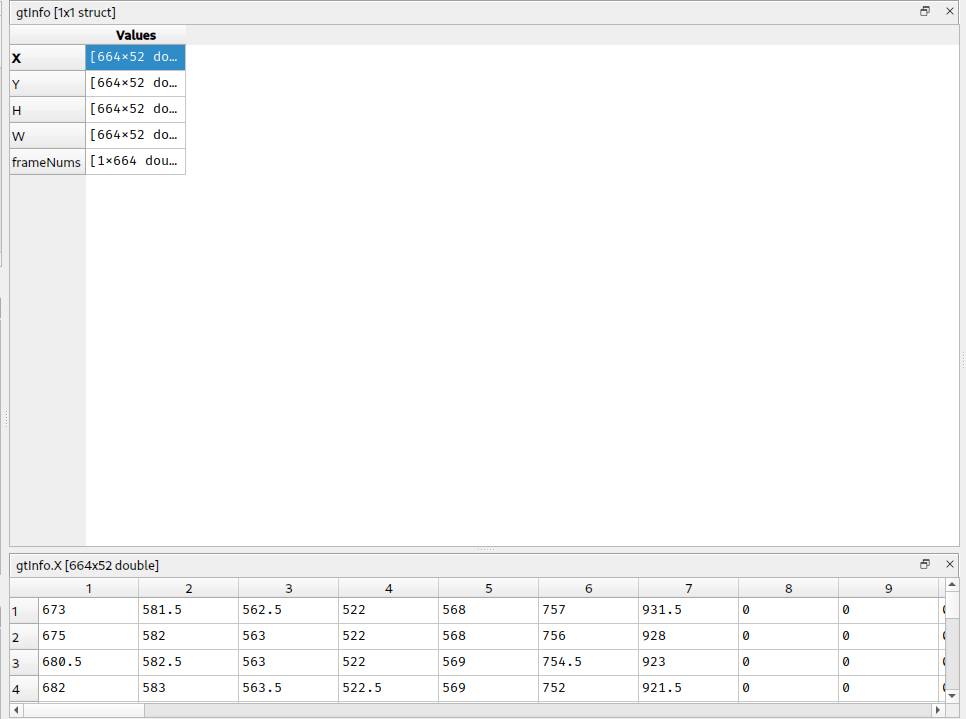
\includegraphics[width=0.8\textwidth]{figures/octave.png}
        \caption{Label data exploration in octave}
        \label{fig:octave-exploration}
    \end{center}
\end{figure}


\section{Used benchmark}

The dataset and the benchmark is described in~\cite{CVIU_UA-DETRAC}. The article also proposes an evaluation protocol for multi-object tracking. A key point is the joint analysis of detection and tracking performance, analysing the effects of the chosen model's precision/recall values (and the underlying confidence threshold setting that influences both) in relation with the tracking performance, as reflected by the MOTA and MOTP score. These relationships are visualized on the PR-MOTA and PR-MOTP curves (See figure~\ref{fig:pr-mota}).

\begin{figure}[h]
    \captionsetup{width=\textwidth}
    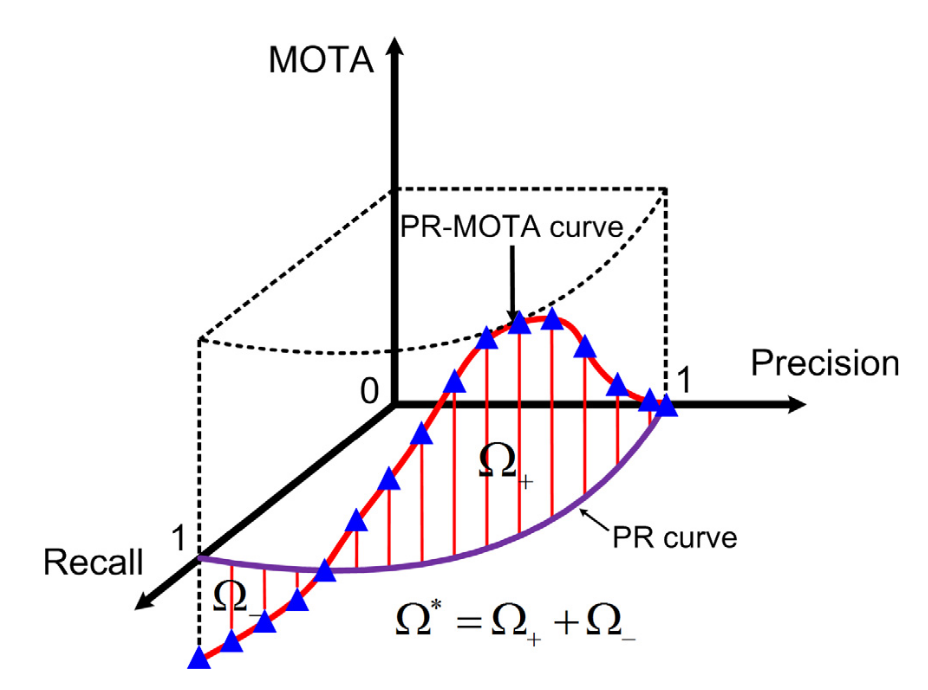
\includegraphics[width=\textwidth]{figures/pr-mota-curve.png}
    \caption{Visualization of the PR-MOTA curve. Image taken from \cite{CVIU_UA-DETRAC}}
    \label{fig:pr-mota}
\end{figure}

The authors argue that, as it is not fair, nor enough to compare the performance of two object detectors based on different points on the PR curve, it is also not enough to determine the maximum point on the PR-MOTA curve, as a good tracker must produce good scores in a wider range of settings. The whole range of the curve must be taken into account in some form, thus the need for a new metric, $\Omega^{*}$, or the \textit{PR-MOTA score}:

\[ \Omega^{*} = \frac{1}{2}\int_{\mathcal{C}} \Psi(p, r) \,d\textbf{s} \]

where $\Psi$ is the MOTA score across the whole dataset at precision $p$ and recall $r$, and we calculate the (approximate value of the) signed area under the PR-MOTA curve as an integral along the PR curve $\mathcal{C}$ (for every $(p, r) \in \mathcal{C}$). Dividing by 2 ensures that the score stays in the interval $(-\infty, 100\%]$. Similar metrics can be defined for the MOTP, FP, FN, IDS, MT and ML scores.

\section{Designing the measurement}

For the measurment, I chose 7 detectors in total: two DETR variants, one with the ResNet50 and one with the ResNet101 backbone, pre-trained on the COCO 2017 dataset. The other 5 were the YOLOv5n (nano), YOLOv5s (small), YOLOv5m (medium), YOLOv5l (large), YOLOv5x (extra large). These differ in the size, as in number of parameters, and this influences the inference times as well.

Each detector was evaluated at 10 confidence thresholds: from 0.0 to 0.9, incremented by 0.1.

To calculate the value defined by the UA-DETRAC benchmark, I had to break the process into multiple steps and assess the best tool for each subtask.

As input data, I had the UA-DETRAC training videos, as frame sequences, and the annotations in MATLAB format.

For my tracker of choice, I could clone the public GitHub repository\footnote{\url{https://github.com/abewley/sort}}, and run the tracker, provided I put the detections in MOT2015 format for each sequence under the \verb|data| folder.

The rest of the steps had to be implemented by me. First, I had to create a model executor that returned the detections from each frame of the video sequences, and served as a adapter-wrapper around both the DETR and the YOLOv5 models, to hide the differences in preprocessing. I invoked this this on all combinations of models, confidence thresholds and sequences. For each unique trio of these, one file has been saved in the MOT15 detection format.

The detections themselves, along with the annotations were enough to calculate the precision-recall curve for each model, aggregating the values for all sequences. For evaluation I used the standard IoU metric for ground truth-prediction distance, with IoU threshold 0.7 (In the code, \verb|max_iou| is set to 0.3, because the library I used considers $1-IoU$ when matching ground truth with prediction. More on that in the relevant subsection). This is not to be confused with the confidence threshold, which is a property of the detector that can be set, and varies. This is a global setting which means that a good prediction can be considered a match to the ground truth box only if their IoU distance is at least 0.7, a reasonable expectation according to my visual intuition.

Next, I ran the SORT script provided in the official repository for each model separately, on every sequence and confidence threshold combination. These were automatically saved in the MOT15 tracking annotation format.

Having the tracking output and the ground truth annotations, I ran the tracking evaluation on every model and confidence threshold combination, aggregating MOTA values for all sequences. The evaluation IoU threshold was set to 0.7, like at the detection evaluation.

Given both the precision-recall curves for every model (where both precision and recall are a function of the confidence threshold), and the MOTA values for every model and confidence threshold combination, I could finally calculate the PR-MOTA scores for each model.

A visual overview of the process above can be seen in figure~\ref{fig:workflow}. Detailing of the individual design choices made at each step can be found in the following subsections. At some of the steps, I implemented visualizations as a way to spot possible errors in implementation that could compromise the whole measurement. 

The language I used was Python 3.10, the inference times were recorded under Linux, on a desktop PC with an AMD Ryzen 3800X processor, 32 Gigabytes of RAM and an RTX3060Ti graphics card with 8 Gigabytes of VRAM. 

\begin{figure}[h]
    \captionsetup{width=\textwidth}
    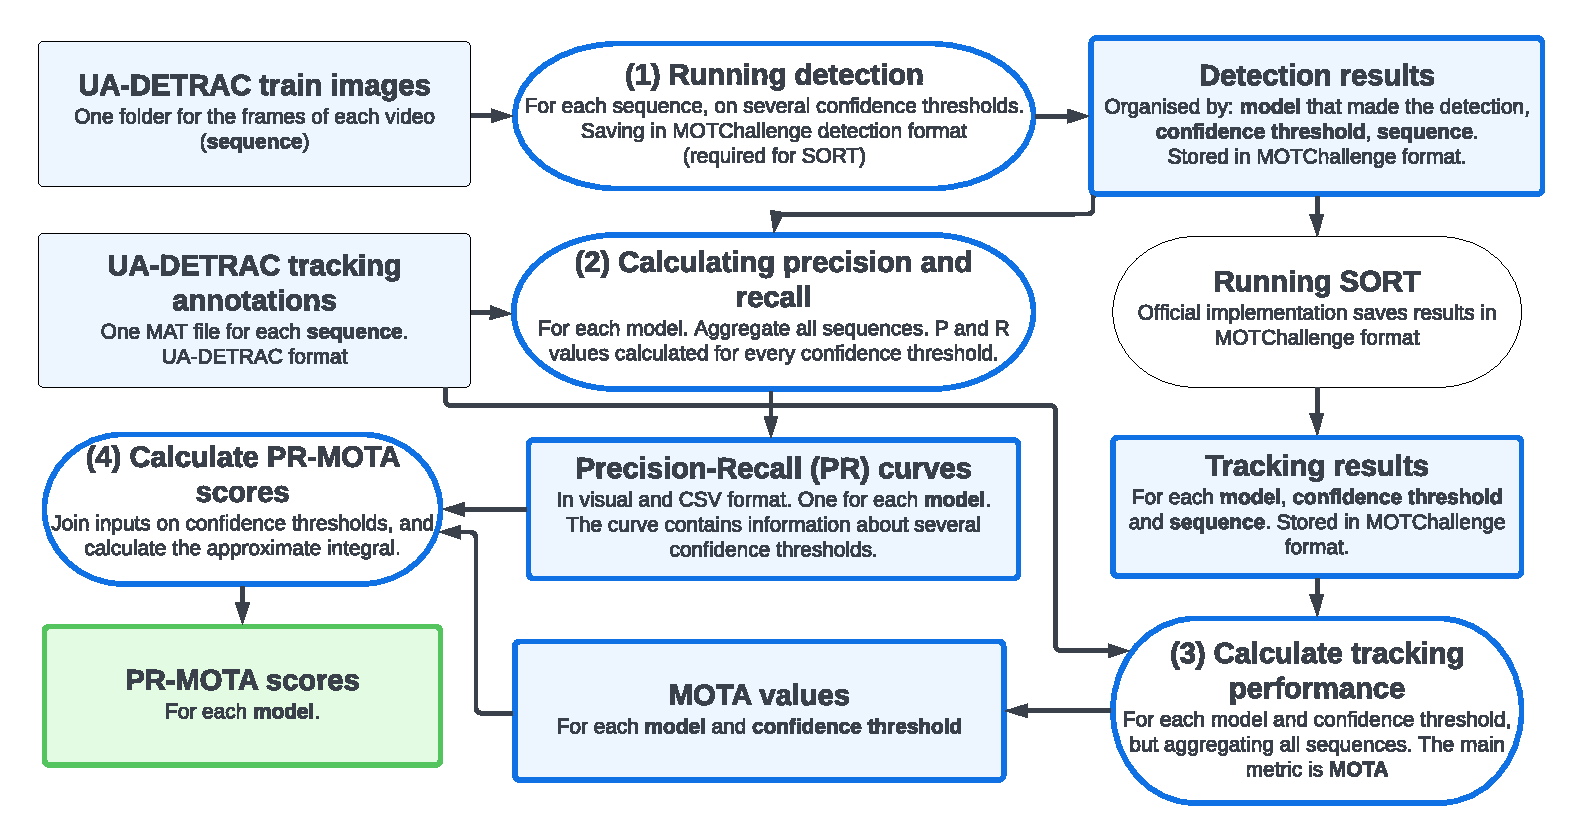
\includegraphics[width=\textwidth]{figures/workflow.pdf}
    \caption{Flowchart visualization of my workflow. The blue rectangles denote data, rounded rectangles denote processing steps. Blue outline means that part of the workflow was implemented by me, or the data was generated in the process. No blue outline means either the data is from an external source, or the processing step involved using entirely external code.}
    \label{fig:workflow}
\end{figure}

\subsection{Running the detections}

In order to evaluate the aforementioned models on images, I had to find the easiest way to load the pretrained weights for each model.

For the DETR, the \verb|transformers| Python package by Huggingface\footnote{\url{https://huggingface.co/docs/transformers/index}} provides the easiest API, with simple pre- and postprocessing (including confidence thresholding and converting from logits to probability distributions), and also provides a way to download pretrained weights. Under the hood, \verb|transformers| uses a PyTorch \verb|torch.nn.Module|, so sending it to the GPU is similar to all Torch modules. Also theoretically loading from Torch Hub was also a possibility, but the pre- and postprocessing tasks would have been messier.

As for the YOLOv5 model, it can be loaded directly from Torch Hub, and its input format is way more flexible, so lists of images (for the inference, I used batches of size 1), but even image links can  be fed to it directly.

To hide the differences between these two approaches, I implemented an adapter class for them, and also added visualization capabilities to spot possible errors in the interpretation of data (for example, assuming wrong bounding box format).

I also wanted to meausre average inference times to show a picture about the real time capabilities of each detector. All inference happened on the GPU, so due to the asynchronous nature of the Torch CUDA operations, measuring elapsed time on CPU was out of the question. The appropriate time measuring method, as suggested on the official Torch forums\footnote{\url{https://discuss.pytorch.org/t/how-to-measure-time-in-pytorch/26964}} was through the \verb|torch.cuda.Event| object. I took the elapsed GPU time between the moment of feeding the inputs until recieving the logits, but this didn't include copy times between the RAM and VRAM, neither the postprocessing steps (calculating probability distributions with softmax, confidence thresholding).

Timing results can be seen in table~\ref{tab:inference-times}. All code to reproduce the results can be found on the GitHub repository of my thesis\footnote{
    See \url{https://github.com/peter-i-istvan/bsc-thesis}, under \texttt{tracking/run\_detection.py}.
}.

\begin{table}[h]
    \begin{tabular}{|c|c|c|c|c|c|c|c|}
        \hline
         & yolov5n & yolov5s & yolov5m & yolov5l & yolov5x & detr-resnet-50 & detr-resnet-101 \\
        \hline
        \hline
        avg (ms) & 7.38 & 7.38 & 8.99 & 12.00 & 20.88 & 43.98 & 64.53 \\
        \hline
        std (ms) & 1.16 & 0.24 & 0.24 & 0.18 & 0.27 & 0.80 & 0.66 \\
        \hline
        \hline
            FPS & 135.5 & 135.5 & 111.2 & 83.3 & 47.89 & 22.73 & 15.49 \\
        \hline
    \end{tabular}
    \caption{Average inference times on GPU and their standard deviation (expressed in miliseconds) for each model, after running on every sequence.}
    \label{tab:inference-times}
\end{table}

\subsection{Calculating precision and recall}

Next, I had to calculate precision and recall curves for the detections. To do this, for every model and confidence threshold pair, I had to sum all true positives, false positives and false negatives in every sequence. For the theoretical definition of these, not only in the general meaning, but in the case of object detection, where assignment between ground truth and predicted boxes is not always trivial (the Hungarian bipartite graph matching algorithm solves this ambiguity), see chapter one.

For the concrete implementation, I took a `sideways' approach, but one that could be mostly reused later in calculating the MOTA score as well. The \verb|motmetrics| Python package\footnote{\url{https://pypi.org/project/motmetrics/}} provides handy tools for calculating MOT metrics, like those in CLEAR MOT. Specificaly, it gives us an \textit{accumulator} object that must be initialized before evaluating on a seqence, then for each frame, its \verb|update()| function must be called to update its state. In the arguments, one must provide ground truth IDs and predicted IDs, as well as a distance matrix that expresses the distance between ground truth box \textit{i} and prediction box \textit{j}. In theory, \verb|motmetrics| is distance-agnostic, which means that any kind of distance can be supplied, but I used the IoU box distance metric, which is one of the most popular evaluation metrics both for object detection and multiple object tracking. \verb|motmetrics| provides functions for calculating all popular metrics, so incorporating IoU calculation into my code was easy.

In its update step, the accumulator takes the input arguments, and in the first parts, it is not at all concerned with the IDs provided, but calculates the best ground truth box-to-prediction assignment with the Hungarian algorithm. This is the very exact action that is needed at detection evaluation as well, this is why we `piggy-backed' tracking evaluation. Based on this assignment, it generates \verb|MATCH|, \verb|MISS| and \verb|FP| events, which correspond to true positives, false negatives and false positives respectively.

In the next steps, if we provided valid prediction IDs (a.k.a our hypotheses for the identities of the tracked objects), the accumulator would also record possible mistakes with regard to identity confusion, like identity swaps. However, considering that the MOTChallenge format defines -1 as the ID field when saving only detections, not tracking results, technically we tell the accumulator that all found boxes correspond to our object -1, which makes the rest of this step absolute rubbish, but it does not influence the events already recorded in the first step, and in the first steps of all future update calls.

After finishing a sequence, the script extracts the number of relevant events, and adds them to all the previously calculated occurrences of true positives, false negatives and false positives for that model-confidence threshold pair. At the end of this, we will have a mapping counting all of these for every sequence. Then I iterate through all model-confidence threshold pairs, calculate the precision and recall values given by the formulas:
\[P = \frac{TP}{TP + FP}\]
\[R = \frac{TP}{TP + FN}\]

Finally, I save them as CSV files. The result can be seen in tables~\ref{tab:p_curve} and~\ref{tab:r_curve}.

\begin{table}
    \begin{centering}
    \begin{tabular}{|c||c|c|c|c|c|c|c|}
        \hline
        CT & D101 & D50 & YL & YM & YN & YS & YX \\
        \hline
        \hline
        0.9 & 0.52 & 0.47 & 0.93 & 1.0 & 1.0 & 0.90 & 0.64 \\
        \hline
        0.8 & 0.45 & 0.41 & 0.54 & 0.61 & 0.83 & 0.61 & 0.49 \\
        \hline
        0.7 & 0.40 & 0.37 & 0.54 & 0.51 & 0.68 & 0.52 & 0.46 \\
        \hline
        0.6 & 0.36 & 0.33 & 0.51 & 0.46 & 0.53 & 0.45 & 0.44 \\
        \hline
        0.5 & 0.33 & 0.30 & 0.46 & 0.42 & 0.42 & 0.39 & 0.41 \\
        \hline
        0.4 & 0.30 & 0.28 & 0.40 & 0.37 & 0.34 & 0.32 & 0.36 \\
        \hline
        0.3 & 0.28 & 0.26 & 0.33 & 0.31 & 0.28 & 0.27 & 0.30 \\
        \hline
        0.2 & 0.25 & 0.23 & 0.30 & 0.28 & 0.25 & 0.24 & 0.27 \\
        \hline
        0.1 & 0.21 & 0.21 & 0.30 & 0.28 & 0.25 & 0.24 & 0.27 \\
        \hline
        0.0 & 0.19 & 0.18 & 0.30 & 0.28 & 0.25 & 0.24 & 0.27 \\
        \hline
    \end{tabular}
    \caption{The precision curve of the models. CT is confidence threshold, D101 and D50 is DETR-Resnet 101 and 50, while YL, YM, YN etc. are the yolo versions.}
    \label{tab:p_curve}
    \end{centering}
\end{table}

\begin{table}
    \begin{centering}
    \begin{tabular}{|c||c|c|c|c|c|c|c|}
        \hline
        CT & D101 & D50 & YL & YM & YN & YS & YX \\
        \hline
        \hline
        0.9 & 0.63 & 0.57 & 0.03 & 0.01 & 0.00 & 0.02 & 0.12 \\
        \hline 
        0.8 & 0.69 & 0.65 & 0.41 & 0.34 & 0.13 & 0.36 & 0.46 \\
        \hline 
        0.7 & 0.71 & 0.68 & 0.59 & 0.52 & 0.41 & 0.56 & 0.60 \\
        \hline 
        0.6 & 0.73 & 0.69 & 0.69 & 0.63 & 0.52 & 0.66 & 0.69 \\
        \hline 
        0.5 & 0.73 & 0.71 & 0.76 & 0.72 & 0.60 & 0.72 & 0.76 \\
        \hline 
        0.4 & 0.74 & 0.71 & 0.81 & 0.79 & 0.66 & 0.77 & 0.81 \\
        \hline 
        0.3 & 0.75 & 0.72 & 0.84 & 0.84 & 0.70 & 0.80 & 0.84 \\
        \hline 
        0.2 & 0.75 & 0.72 & 0.86 & 0.86 & 0.72 & 0.81 & 0.86 \\
        \hline 
        0.1 & 0.76 & 0.73 & 0.86 & 0.86 & 0.72 & 0.81 & 0.86 \\
        \hline 
        0.0 & 0.76 & 0.73 & 0.86 & 0.86 & 0.72 & 0.81 & 0.86 \\
        \hline
    \end{tabular}
    \caption{The recall curve of the models. CT is confidence threshold, D101 and D50 is DETR-Resnet 101 and 50, while YL, YM, YN etc. are the yolo versions.}
    \label{tab:r_curve}
    \end{centering}
\end{table}

Running this took 1 hour and 8 minutes on my machine. For implementation, see my GitHub repository\footnote{See \url{https://github.com/peter-i-istvan/bsc-thesis}, under \texttt{tracking/detection\_evaluation.py} for the code, \texttt{p\_curve.csv}, and \texttt{r\_curve.csv} for the curves in }, where the curves are also available, saved in CSV format.

Finally, I wrote a small script that plots precision-recall curves\footnote{\url{https://github.com/peter-i-istvan/bsc-thesis} under \texttt{tracking/plot\_pr.py}. The PNG plots are also there under the root directory.} for each model. The results can be seen in figures~\ref{fig:pr_detr} and~\ref{fig:pr_yolo} in the appendix.

\subsection{Running SORT}

I ran SORT by cloning its repository, applying a small patch to account for divison by 0 at empty detection files (happened with YOLOv5n models for some sequences, at high confidence thresholds), installing the dependencies and issuing the following command:
\begin{verbatim}
    python sort.py --seq_path DETECTIONS_ROOT --phase MODEL --max_age 3
\end{verbatim}

The main hyperparameters of SORT are \verb|min_hits|, \verb|max_age| and \verb|iou_threshold|, all of them can be supplied to the script by command line parameters.

Minimum hits means the minimum number of consecutive times a new trajectory must be confirmed (by detection `hits' that get assigned to it) to consider it a real one. Its default value is 3, and I left it at that.

Maximum age is the longest consecutive time that a trajectory without detection (if the detector somehow lost the object) can be kept alive. The position predictions are still updated, so the tracker looks for the object a little bit further apart at each frame, in the direction and considering the magnitude of the last known velocity. The default value is 1, but I set it to 3 because it seemed reasonable (based on my experiences in the Project Laboratory course, where similar maximum ages lead to better results).

IoU threshold is the minimum IoU value between the hypothesized current bounding box location of the object (predicted by the Kalman filter) and any detection bounding box that can be matched with it. The default value is 0.3, and I left it at that.

During the consecutive runnings of the script, I recorded the elapsed time and FPS reported by the script for each model. The results are confirming the belief that SORT is a very fast tracker, with the main factor for the tracking framerate in a real time scenario (where detections are not precomputed) being the detection time (almost two orders of magnitude higher than the tracking time at each frame). For the results, see table~\ref{tab:sort-times}.

\begin{table}[h]
    \begin{tabular}{|c|c|c|c|c|c|c|c|}
        \hline
         & yolov5n & yolov5s & yolov5m & yolov5l & yolov5x & detr-resnet-50 & detr-resnet-101 \\
        \hline
        \hline
        Time (s) & 1313.99 & 1155.18 & 482.8 & 599.88 & 611.18 & 654.18 & 668.11\\
        \hline
        \hline
        FPS  & 637 & 725 & 1710.2 & 1391.7 & 1369.1 & 1279.1 & 1253.5 \\
        \hline
    \end{tabular}
    \caption{Statistics reported by the SORT script. The evaluation was done on 60 videos and on 10 confidence thresholds, making a total of 600 detection inputs. The time is the total evaluation time for all 600 inputs. The numbers are aggregated over confidence thresholds, but on lower values, tracking tends to take more time, as the consistent erroneus detections form a high number of false tracks.}
    \label{tab:sort-times}
\end{table}

\subsection{Calculating tracking performance}

After the tracking outputs were ready, I ran the tracking evaluation. The main goal was to calculate MOTA scores, average MOTA for every model-confidence threshold pair, across all sequences. Eventually I ended up calculating more metrics, to see a broader picture about the tracker performance.

For this, I used the \verb|motmetrics| library, similarly to the detection evaluation. I processed each sequence with an accumlator objects, computing several summary metrics at the end. For every model, confidence threshold, sequence trio, I had a summary in the form of a Pandas dataframe, holding all the same metrics. I gathered all these, then aggregated across the sequences, recieving aggregate scores for each model and confidence threshold.

The scores I queried in for each sequence were the \textit{MOTA}, \textit{MOTP}, number of \textit{identity switches}, the number of \textit{mostly tracked trajectories} (80\% or more of it was tracked), \textit{mostly lost trajectories} (20\% or less of it was tracked), and the number of \textit{unique objects}. I aggregated the MOTA and MOTP by averaging (also saving minimum and maximum MOTA score), the rest by calculating the sum of their values.

It is important to mention that I sticked to the original definition of MOTP, introduced in~\cite{Bernardin2008}, meausres average IoU dissimilarity between true positive predicted trajectories and ground truth, and a smaller value is preferable. In some publications, even in~\cite{Bewley_2016}, the value claimed to be MOTP is actually $1-MOTP$, scaled to percentages, so that higher value is better.

Running this took 1 hour and 10 minutes. For implementation, see the GitHub repository\footnote{\url{https://github.com/peter-i-istvan/bsc-thesis} under \texttt{tracking/tracking\_evaluation.py}. The results in CSV format are also available from the root directory of the repository, as \texttt{MODELNAME\_mota.csv}}. Results can be seen in tables~\ref{tab:mota_yn},~\ref{tab:mota_ys},~\ref{tab:mota_ym},~\ref{tab:mota_yl},~\ref{tab:mota_yx},~\ref{tab:mota_detr50},~\ref{tab:mota_detr101} in the appendix. A plot of the average and maximum MOTA across sequences, for each detector category can be seen in figures~\ref{fig:avg-mota} and~\ref{fig:max-mota}.

Unfortunately, the general overall results across all thresholds were not favorable, with the YOLOv5 medium and large versions reaching best tracking results for confidence thresholds around 70-80\%. In terms of average MOTA across all sequences, they both reached 33-35\% at 80\% confidence threshold, while their maximum MOTA reached in any sequence was and 80-81\% at 70\% confidence threshold.

For the DETR models, MOTA scores underperformed their YOLO counterparts by not reaching positive average scores, but reaching peak average MOTA at 90\% confidence threshold. Their best peroformances on any sequence was 69-74\% MOTA at 90\% confidence threshold.

\begin{figure}[h]
    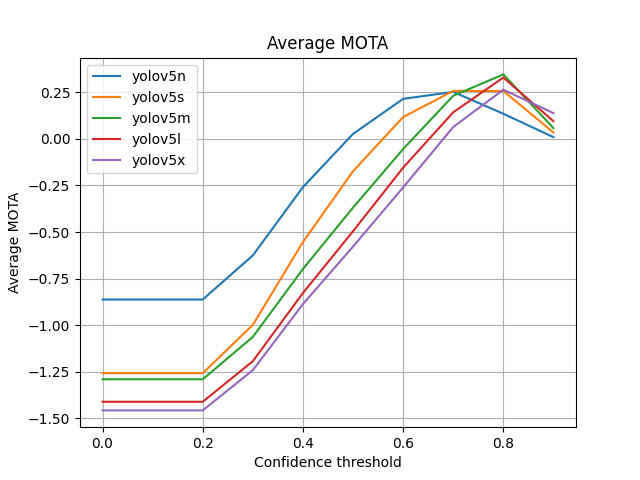
\includegraphics[width=0.49\textwidth]{figures/yolo_mota.png}
    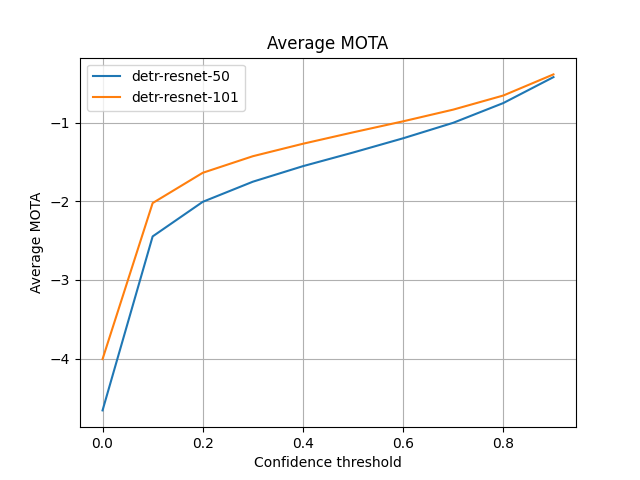
\includegraphics[width=0.49\textwidth]{figures/detr_mota.png}
    \caption{Average MOTA scores for each model.}
    \label{fig:avg-mota}
\end{figure}

\begin{figure}[h]
    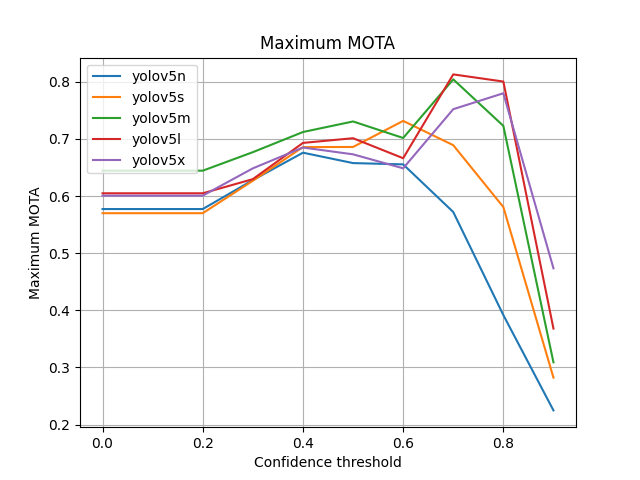
\includegraphics[width=0.49\textwidth]{figures/yolo_max_mota.png}
    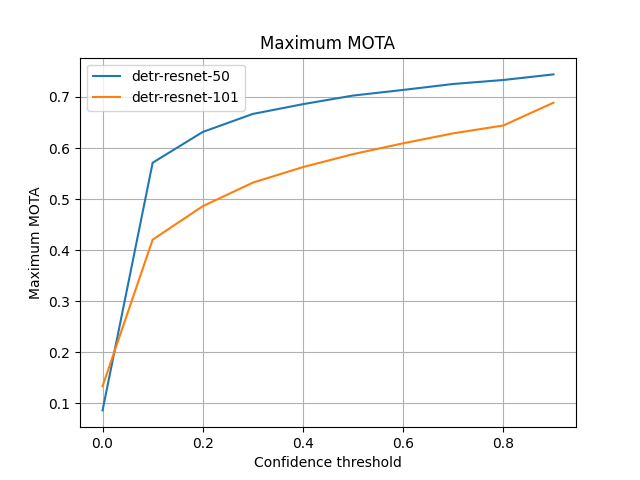
\includegraphics[width=0.49\textwidth]{figures/detr_max_mota.png}
    \caption{Maximum MOTA scores for each model.}
    \label{fig:max-mota}
\end{figure}

\subsection{Calculting benchmark scores}

Finally, I calculated the PR-MOTA score for each detector by joining the previous results along confidence thresholds, using trapezoidal rule approximation to calculate the integral:

\[\int_{\mathcal{C}}{MOTA(\textbf{s})d\textbf{s}} \approx \sum_{t = 2}^{10}{|C_tC_{t-1}|}\frac{MOTA(C_{t-1}) + MOTA(C_t)}{2} \]

where $C_1$, $C_2$, ..., $C_{10}$ are subsequent points on the $\mathcal{C}$ precision-recall curve defined by confidence thresholds between $0$ and $1$ with increments of $0.1$, while $|C_tC_{t-1}|$ denotes the distance between the two points. In practice, for the $1.0$ threshold the detectors supplied no output, so I defined their precision as $1$ (no bad hits) the recall as $0$ (found no true positive), and the $MOTA$ as $0$, in the spirit of the definition of these metrics.

The code for this step can be found, as usual, in the thesis' repository\footnote{\url{https://github.com/peter-i-istvan/bsc-thesis} under \texttt{tracking/calculte\_pr\_mota.py}, and also \texttt{pr\_mota.csv} for CSV results.}. The results can be seen in table~\ref{tab:pr-mota}. They can be considered relatively poor, and indicate that in the bigger part of the $[0;1]$ confidence interval, average MOTA scores are negative. This should be no suprise, because usually one does not trust the detections with confidence below 50\% (I found this to be true empirically, while experimenting with `off-the-shelf' pretrained models like these). The DETR underperforms the YOLO on this metric by a relatively large margin.

\begin{table}[h]
    \centering
    \begin{tabular}{|c|c|c|c|c|c|c|c|}
        \hline
        & D101 & D50 & YL& YM & YN & YS & YX \\
        \hline
        PR-MOTA & -1.33 & -1.51 & -0.42 & -0.37 & -0.19 & -0.33 & -0.46 \\
        \hline
    \end{tabular}
    \caption{PR-MOTA results.}
\label{tab:pr-mota}
\end{table}

The best among the DETR is the one with the ResNet101 backbone. This is not surprising, as the ResNet101 is the larger backbone, which usually means richer feature data to work with.  

Surprisingly, among the YOLO, the nano version had the best score. This was unexpected beacuse overall, the large and medium versions reached the highest scores. It can be somewhat explained looking at~\ref{fig:avg-mota}, where the nano version seems to have the highest signed area under the curve, and it has better performance on low confidence thresholds, but this only shows that the measurement is heavily influenced by how bad the tracking was at lower confidence. In production applications, one would chose a relatively high confidence threshold to start with, so the PR-MOTA score fails to predict future performance in such cases, as here the performance metrics on reasonable confidence thresholds are outweighted during averaging.



\section{Conclusion}

When viewing the final results by my chosen metric, the PR-MOTA score seems poor across all detectors. However, I concluded that, in this case, it is a flaw of the metric itself, which fails to predict usefulness in real life scenarios. As I observed, all the detectors I have tried give useless predictions under the confidence threshold of 50-60\% from the perspective of the SORT tracker. The measure of uselessness is almost irrelevant, but this difference is what caused the YOLOv5 nano to reach best score.

The real best performing object detectors were the YOLOv5 medium and large models, reaching about 35\% average MOTA on reasonable, 70-80\% confidence thresholds (in addition, the MOTA results obtained here show high variance, because even considering the average of 35\%, on some sequences it varies from -90\% to +80\% - see appendix). This is actually on par with SORT performance as first published in 2016~\cite{Bewley_2016} across various kinds of datasets, but considering the time passed since the publication, it would seem that the apparent improvement in detector quality in the meantime (from 2016 to 2020, publication date of the inspected models) has not brought great improvement in tracking performance. However, I suspect that this more related to the inspected detectors, and the way I evaluated them, than to the usefullness of SORT.

Both detectors were pretrained on the COCO 2017 dataset, a large and rich database of annotated images and numerous object classes, on a long and resource-hevy training regimen, the kind of which I could not replicate. Even though I only used three vehicle categories, the models themselves are capable of recognising much more, and during training the goal is to find all classes, and in all non-iconic poses too. Compared with the object feature distribution of the UA-DETRAC, COCO is richer both in number of object classes and in the context of the cars (the UA-DETRAC contains only vehicles engaged in road traffic, and from fixed camera angles). This generality of the COCO-trained models might hurt specific performance on UA-DETRAC, this is why fine-tuning on similar datasets, or even the vehicle subset of COCO would have helped. In this regard, considering the smaller visual diversity of UA-DETRAC, models from 2016 trained on it specifically can indeed perform on par with models from four years later, trained on COCO, even though the former models would score worse when trained on COCO, because of the inherent inferiority.

Regardless of the above, from the perspective of the original goal, the measurement provided insightful results in comparing a specific convolutional and and a specific Transformer-based object detector that were introduced roughly at the same time. Measurements from all aspects show that the COCO-trained YOLOv5 models outperform the COCO-trained DETR by a large margin when used in multiple vehicle tracking scenarios. It outperforms not only in quality, but in speed, as the inference and tracking times show that all versions of YOLOv5 are capable of real-time detection and tracking (when evaluated on my system), defined as 30 FPS or above, while the DETR versions are not, they are on average 3 to 6 times slower.

This concludes my inquiry, but it is needed to mention that from 2020 until the present, Transformer-based visual models, and object detectors specifically have seen great improvement, with introduction of new models like the Swin Transformer, Deformable DETR, Group DETR, GRiT, DINO etc. When inspecting leaderboards on Papers with Code\footnote{A popular online collection of machine learning publications, links to official codebases and benchmark results for comparison. See \url{https://paperswithcode.com/sota/object-detection-on-coco}}, it seems that evaluated on the COCO test set, the best of these currently outperform the YOLO series, but most convolutional object detectors as well. The only category where YOLO still has an edge is quality to speed ratio, as for real-time object detection, YOLOv7 is currently the leading model, outperforming fast visual Transformers like Swin.\footnote{\url{https://paperswithcode.com/sota/real-time-object-detection-on-coco}}.
